\chapter{Inleiding}
\label{hoofdstuk:I}
%In dit hoofdstuk wordt het werk ingeleid. Het doel wordt gedefinieerd en er
%wordt uitgelegd wat de te volgen weg is (beter bekend als de rode draad).

%Als je niet goed weet wat een masterproef is, kan je altijd
%Wikipedia\cite{wiki} eens nakijken.

\section{Probleemstelling}
Een van de meest voorkomende problemen voor muzikanten is de zogenaamde \textit{writer's block}. Dit fenomeen waarbij je als muzikant merkt dat je de hele tijd op hetzelfde melodietje uitkomt en maar niet met iets nieuw kan komen kan zeer frustrerend zijn. Daarom zou het handig zijn als er een tool zou bestaan die je als het ware de inspiratie kan geven die je nodig hebt om deze \textit{writer's block} te doorbreken. Een mogelijke oplossing voor dit probleem wordt in deze thesis onderzocht. Hier gaat het dan om het transformeren van reeds gekende melodie\"en tot nieuwe melodie\"en.

\section{Vergelijking met voorgaand onderzoek}
Onderzoek naar het bekomen van nieuwe melodie\"en waarbij gebruik gemaakt wordt van een computer is niet nieuw. Al gedurende tientallen jaren is er veel werk geleverd op het vlak van muziekgeneratie, waarbij het de bedoeling is om een muziekstuk te genereren waarbij vertrokken wordt van een lege partituur. Dit wordt gedaan rekening houdend met de regels uit de muziektheorie en vaak probeert men er ook een vorm van repetitiviteit en herkenning in te brengen zoals vaak ook het geval is in hedendaagse muziek. Een groot probleem dat echter altijd terugkwam was dat het heel moeilijk was om een goede verhouding te vinden tussen twee heel belangrijke eigenschappen van de muziek, namelijk verwachting en verrassing van de luisteraar. Een muziekluisteraar heeft namelijk een bepaald verwachtingspatroon voor het onmiddellijke vervolg van een melodie. Dit verwachtingspatroon strookt vaak met de regels van de muziektheorie. Wanneer deze regels dan weer te nauwgezet gevolgd worden, wordt het muziekstuk als saai ervaren, er is dus nood aan een zekere verrassing in de melodie. Te veel onverwachte wendingen worden dan weer als frustrerend gezien, kortom, het is van cruciaal belang om een goed evenwicht te vinden tussen deze twee waarden. En dit blijkt zeer moeilijk te verwezenlijken vanuit een muziek generatie-standpunt.\\

\section{Doelstelling}
In deze thesis wordt een onderzoek gevoerd naar de generatie van nieuwe melodie\"en vertrekkende van originele melodie\"en. Deze originele melodie\"en worden bij aanname verondersteld te voldoen aan de eisen van verrassing en verwachting. In deze thesis worden specifiek melodische transformaties onderzocht. Deze transformaties zullen gebaseerd zijn op wiskundige reeksen. Hierbij gaat men voor elke noot in de oorspronkelijke melodie de toonhoogte aanpassen volgens een bepaald patroon. Als voorbeeld om het concept te verduidelijken kan figuur \ref{figuur:fibo} dienen. In deze figuur wordt met behulp van de rij van fibonacci een originele melodie getransformeerd tot een nieuwe. Er wordt getracht zo een transformatie te zoeken zodat de nieuw bekomen melodie nog steeds consonant is (nog steeds goed klinkt). Er zal ook onderzocht worden onder welke omstandigheden een transformatie al dan niet een consonante melodie oplevert. Om te bepalen of een nieuwe melodie goed klinkt is er ook nood aan een objectieve beoordeling van deze melodie\"en. Er wordt dus ook aandacht besteed aan het opstellen van een model dat hiervoor kan dienen. Een model dat zo goed mogelijk kan beoordelen of een gegeven melodie al dan niet, en in welke mate, consonant is. Het voordeel van het werken met transformaties in plaats van met generatie is dat men op deze manier nog een deel van de eigenheid van het originele werk kan behouden en het bekomen werk hierdoor ook minder artificieel zal overkomen bij de luisteraar.

\begin{figure}[!ht]
  \centering
  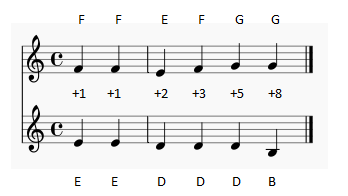
\includegraphics[width=0.5\textwidth]{0_Inleiding/fibo}
  \caption{Melodische transformatie m.b.v. rij van Fibonacci: Noten op de bovenste notenbalk liggen respectievelijk 1,1,2,3,5,8 halve tonen hoger dan op de onderste notenbalk.}
  \label{figuur:fibo}
\end{figure}

\section{Assumpties en beperkingen}
Op een onderdeel van hoofdstuk \ref{hoofdstuk:OBM} na, behandelt deze masterproef enkel muziek met precies \'e\'en melodielijn. Meerstemmige muziek waarbij meerdere noten tegelijkertijd gespeeld kunnen worden, wordt in deze thesis dus niet behandelt. Verder worden alle testen uitgevoerd op een corpus (Essen corpus \cite{url:essen}) bestaande uit muziekstukken van het `folk'-genre. Tot slot zal ook telkens wanneer een transformatie uitgevoerd is, er vanuit gegaan worden dat het originele muziekstuk telkens voldoet aan de algemene voorwaarden waaraan een muziekstuk moet voldoen, zodat zijn score in het voorgestelde model telkens ook als referentie kan dienen voor zijn getransformeerde versie. 

\section{Overzicht van de tekst}
In het eerstvolgende hoofdstuk, hoofdstuk \ref{hoofdstuk:MA} wordt een korte inleiding gegeven tot de muziektheorie. Hierin worden enkel deze elementen behandeld die relevant zijn voor de rest van deze thesis. Vervolgens zal er een besproken worden hoe een bepaald muziekstuk objectief kan beoordeeld worden, dit zal gebeuren in hoofdstuk \ref{hoofdstuk:OBM}. In hoofdstuk \ref{hoofdstuk:MT} worden verschillende melodische transformaties toegelicht en met elkaar vergeleken. Vervolgens zal hoofdstuk \ref{hoofdstuk:ETT} twee algoritmes beschrijven. Deze algoritmes kunnen gebruikt worden om gegeven een aantal toegestane transformaties en een oorspronkelijke melodielijn, de meest waarschijnlijke getransformeerde melodielijn terug te geven. Hierna zullen een aantal experimenten, alsook hun resultaten besproken worden in hoofdstuk \ref{hoofdstuk:ER}. Tot slot wordt er in hoofdstuk \ref{hoofdstuk:B} nog teruggekeken op het geleverde onderzoek in een samenvattend besluit. Er wordt ook nog beschreven welk verder onderzoek zeker nog interessant zou kunnen zijn binnen dit onderwerp. 

%%% Local Variables: 
%%% mode: latex
%%% TeX-master: "masterproef"
%%% End: 
